\documentclass[a4paper]{jpconf}
\usepackage{graphicx}

\begin{document}
\title{Application of a novel machine learning algorithm in gravitational wave transient noise identification}
\author{Ruaridh O'Donnell}
\ead{1002205o@student.gla.c.uk}
\begin{abstract}
    Due to the low amplitude of gravitational waves, data from gravitational wave detectors is high in noise. A large portion of this noise is transient and of high amplitude. It can be confused with real gradational wave signals. This project is an investigation into whether a recent machine learning algorithm (NuPIC) would be of use in classifying transients. A detailed description of how this algorithm functions is given. The algorithm was trained on a sine gaussian model and tested to see how well it could differentiate the trained signal from background gaussian noise. Up to an SNR of 5.1 it was able to differentiate the signal well, but for higher levels of noise it could not. Notes were made on how the algorithm deals with noise. These could be helpful in future work.
\end{abstract}

%%%%%%%%%%%%%%%%%%%%%%%%%%%%%%%%%%%%%%%%%%%%%%%%%%
\section{Overview}
	The aim of this work was to look at the possible use of a a novel unsupervised machine learning algorithm in the search for gravitational waves. The algorithm, NuPIC is used commercially in detecting patterns in time series data. Gravitational wave detectors produce a lot of transient high amplitude noise in their output. This is often correlated with data that measures other aspects of the detector. It was thought that this algorithm could detect these patterns.
	
	The algorithm was tested to see how well it could differentiate a known signal from noise. More work is needed to verify if the algorithm can work with real data.
    
%%%%%%%%%%%%%%%%%%%%%%%%%%%%%%%%%%%%%%%%%%%%%%%%%%
\section{Background On Gravitational Waves and Detectors}
Advances in astronomy typically follow advances in detector technology. Telescopes tuned to wavelengths of light outside the visible spectrum have produced many discoveries beyond what was known only from visible light telescopes. Gravitational waves are predicted to be emitted by many astronomical bodies. If they can be detected then they provide a new method of discovery that is substantially different from electromagnetic radiation.

Detecting gravitational waves generates many technical challenges and thus the detectors are complex. This section will cover the relevant feature of the detectors for this project and also cover some of the ways in which machine learning has been used in this field in the past.

	\subsection{Gravitational wave detectors}
		The gravitational wave detectors in use today are fundamentally Michelson interferometers. The mirrors at either end of the arms are mounted on test masses that move when gravitational waves pass. The output that measures the wave can be thought of as a time series of the power output of the interferometer. In reality modern advanced detectors (such as Advanced LIGO) are considerably more complex but the details do not need to be understood.

	The waves detectable from earth have an extremely small effect on the test masses. The detectors need to have advanced noise removal so much of the work in building the detectors has gone into this. However despite the efforts much noise still remains in the signal. This noise can be broadly split into gaussian noise and glitches. Where a glitch means is any high amplitude transient noise. The glitches can be mistaken for real gravitational wave signals.

	\subsection{Past attempts at using machine learning methods in gravitational wave searches}
		Machine learning methods are starting to be used in the field of gravitational wave searches. This section contains a summary of some recent efforts. It should be noted that the algorithms used here are substantially different in operation to NuPIC, the algorithm used in this project.

		\subsubsection*{Inferring Core Collapse Supernova Physics with Gravitational Waves [5]}
			There are different possibilities for how supernova evolve. Each produces a different pattern in the gravitational wave signal. However the waveforms vary enough in each class that that cross-correlation would be impractical. So this paper proposes a method for categorising a signal measured in LIGO into one of the three supernova types using principle component analysis and Bayesian statistics. Principle component analysis has some similarities to the way NuPIC operates.
			
		\subsubsection*{Noise Artefact Removal Using Machine learning with Gravitational Waves [2]}
			Glitches occur frequently enough that they show up in concurrence between two detectors. This causes problems when trying to detect gravitational waves across multiple detectors. Glitches often often occur in correlation with other readings taken from the detector. Hence automated machine learning methods can be used to distinguish them from real gravitational wave signals.

			Data was split into two categories. The first; glitches that weren't gravitational waves, i.e. glitches that didn't have any coincidence in other detectors. This was composed of all glitches that were measured, with the assumption that this set contained no gravitational signals. The other was clean data composed of random samples from when the gravitational wave channel was quiet.

			Similar performance was achieved using several different algorithms, suggesting that any improvements would be from including additional data in the classification.

		\subsubsection*{Application of Artificial Neural Network to Search for Gravitational-Wave Signals Associated with Short Gamma-Ray Bursts [4]}
			A fairly basic application of artificial neural networks to categorise glitches.
		
%%%%%%%%%%%%%%%%%%%%%%%%%%%%%%%%%%%%%%%%%%%%%%%%%%
\section{NuPIC: A Novel Machine Learning Algorithm}
	The Numenta Platform for Intelligent Computing (NuPIC) is the machine learning algorithm used in this project. It was developed privately by the company Numenta for use in analysis of streaming data. As of January 2014 it is in use in a commercial product ``Grok'' but the core algorithm has been open sourced.
		
	This section will go over the main features of this algorithm, followed by a more detailed overview of it's inner workings. This will be illustrated with a simple example. Finally the specific implementation details used in this project will be covered as well as a short analysis of the noise characteristics of the algorithm.

	\subsection{Backround}
		Machine learning algorithms automatically learn patterns in collections of data. This automatic discovery of the underlying statistics in data make them useful across a wide class of domains. Most algorithms operate in a similar manner. They are trained on a collection of data until the patterns are discovered, and then they are used to evaluate new data (that was not in the training set). For example, a collection of vectors grouped together into classes can be used by a KNN classifier. A new vector can be evaluated by this algorithm to see which class it belongs to. There is a wide variety in how machine learning algorithms carry out this process. NuPIC was modelled on a theory of how the neocortex (a part of the mammalian brain) functions. This theory is called Hierarchical Temporal Memory (HTM).
		
		The neocortex is the part of the brain associated with higher intelligent thinking and long term memory. It consists of a sheet across the surface of the brain, approximately 2 mm thick, composed of around six layers. Different areas of the sheet carry out different functions (image processing, language, higher level thought, etc). The neocortex is has very regular structure of cells across these different areas. Vernon Mountcastle propositioned that despite the different functions, the neocortex is running the same algorithm across all areas. This is the basis of NuPIC. It is the very first part of an implementation of this algorithm.
	
	\subsection{Main features of NuPIC}
		Most machine learning algorithms have a training phase, where they process the data and learn its statistics. Once this phase is over the algorithm does not change. NuPIC operates in a slightly different manner that has more in common with biological brains. There is no distinct training phase, instead the data is fed in as a sequence and learning is continuous. For example a time series is fed in sample by sample, with learning happening after every sample.
		
		NuPIC is also unsupervised. Supervised machine learning algorithms try to evaluate data against predefined labels. A common example would training on a collection of images of animals, each labeled with the type of animal. Then the algorithm would evaluate a new image of an animal and come up with its type. NuPIC instead categorises data into categories it chooses. This is how biological brains operate.
		
		As well as learning on each sample, NuPIC forms predictions. This is a major part of the background HTM theory. They happen all the time in the brain and play a role in feedback, stability of representations, robustness to noise and expectedness of input. The import features of prediction here are its role in selecting context. When data is fed into NuPIC, it is classified, and a prediction of the next input is formed. This prediction is then used to help classify the next input. This process is detailed in the next section. Prediction allows one to say how unexpected the input is, or how anomalous it is. This anomaly detection was used in the glitch detection.
		
		Internally NuPIC is a neural network. However it the details of this network are more complex than neural networks commonly used.
		
	\subsection{Algorithm details}
		This section borrows heavily from the description in the Numenta white paper which contains a more thorough explanation of the algorithms complete with pseudocode. NuPIC undergoes three steps each time a sample of data is fed in. These are:
		\begin{enumerate}
			\item Form a sparse distributed representation of the input
			\item Form a representation of the input in the context of previous inputs
			\item Form a prediction based on the current input in the context of previous inputs
		\end{enumerate}
		
		\subsubsection{Step 1: Form a sparse distributed representation of the input}
			This step has two subsets. First the input (which in this case could be a sample form a time series, a real number) is converted to a binary vector. This is called encoding. It is not part of the core algorithm but it is necessary to convert the data type of the input into a format that can be used in subsequent steps. It follows that there are different encoders for different data types. For the case of real numbers as used in this project the ``scalar encoder'' was used. A value is converted to a binary vector with a section of on bits in a background of off bits. See fig \ref{fig:scalarEncoder} for details. The dimension of the vector and the number of on bits are parameters that do not change.
			
%:FIG:scalarEncoder
%			\begin{figure}
%				\centering
%				\input{scalarEncoder.eps_tex}
%				\caption{This shows how the scalar encoder maps real numbers to binary vectors. The binary vectors are represented by a line of boxes with white being $0$ and black being $1$. Each binary vector represents an interval of real numbers, so close numbers will map to the same vector. Note that this example only encodes numbers between $0$ and $10$. The width of the vector and the length of the on bits can be set as parameters. Note how numbers close together result in vectors with low Hamming distance.}
%				\label{fig:scalarEncoder}
%			\end{figure}
			The next step is to convert this binary vector to a small set of active \emph{columns} contained in a larger set of inactive ones. Consider the structure in fig \ref{fig:structureDiagram}. The input binary vector from the previous step is input at the bottom. Then, in a process called spatial pooling, a set of columns become active (usually about 2\% of the total number of columns). This set of columns is the sparse distributed representation of the input vector. SDRs have many useful properties which explain why this step is necessary. For example to differentiate each SDR in a set of SDRs it is not necessary to compared each bit. It is possible to check only a few and still get a low probability of mismatch. This reduces the computations that must be performed. Further, this property allows superpositions of two or more SDRs to be formed by or-ing their bits together. The chance of two random SDR overlapping significantly is extremely small. This property proves useful in step 3 (section \ref{step3}).
			
%:FIG:structureDiagram
%			\begin{figure}[h]
%				\centering
%				\input{structureDiagram.eps_tex}
%				\caption{The internal structure of NuPIC}
%				\label{fig:structureDiagram}
%			\end{figure}
			Referring back to the structure diagram (fig \ref{fig:structureDiagram}), each column has a number of synapses. connecting it to a large portion of the input space. Each synapse can be either active or inactive (on or off). An active synapse, permits the information to pass from the input to its column. In the spatial pooling process the following happens: For each column you add up the input bits connected to the column by active synapses. This results in an integer ``score'' for each column. Then, using this score, the top few columns are chosen to be made active. With the number chosen so that 2\% of columns become active. This process is illustrated in fig \ref{fig:algorithmDiagramStep1}. Each column can be thought of as corresponding to a ``pattern'' in the input. The set of active columns represents the input in terms of these ``patterns''. Much like a vector can be decomposed into a combination of orthogonal basis vectors.
			
			At this step learning occurs but it will not be covered here in detail. The learning process modifies the synapses. Each synapse has an associated real number named \emph{permanence}. This is modified during learning and it is this number that decides wether the synapse should be active or inactive.

		\subsubsection{Step 2: Form a representation of the input in the context of previous inputs}
			This step activates a set of \emph{cells} within each of the columns activated in the last step. Each column is composed of a number of cells which can either be active or inactive. The active columns represent the input, whereas the active cells will represent the input in the context of previous inputs. This is important as an input can mean different things in different contexts. This is illustrated in the Numenta White Paper: In the spoken sequence of words ``I ate a pear'' and ``I have eight pears'' the words ``ate'' and ``eight'' sound exactly the same; they are the same input. Yet, given the context, it is clear they mean different things.
			
			Cells are activated as follows: In every active column, each cell is activated if the cell was in a \emph{predicting} state in the time step before. If a column is active but none of its cells are in a predicting state, then all the cells are made active. This process is shown in fig \ref{fig:algorithmDiagramStep2}. Predicting cells are explained in the next step. When all the cells in a column become active this represents an input when the context is not known. Since each cell represents a different context, they are all activated.
			
		\subsubsection{Step 3: Form a prediction based on the current input in the context of previous inputs}\label{step3}
		The previous step referred to cells being in a \emph{predicting} state. This step calculates which cells should be in the predicting state. Note that the result here will be used in the next time step of the algorithm.
		
		Cells are chosen to become predicting in a manner similar to the way columns are chosen to be active in step 1. The details are not as important, but each cell has a collection of synapses (of the same type mentioned in step one) connecting it to other cells. A score for each cell is calculated by summing active cells that are connected by active synapses. If a score crosses a threshold then the cell becomes predicting. The result of steps 2 and 3 is that cell activations follow each other in learned sequences. Synapses are formed from a cell to other cells that commonly become active on the time step before. So if two inputs commonly follow one another, $A$ then $B$. Cells representing input $B$ will form connections to cells representing input $A$. Hence when input $A$ occurs, and the corresponding cells become active, the cells corresponding to input $B$ become predicting.
		
		This behaviour can be used to measure how unexpected an input is. The \emph{anomaly score} is calculated equation \ref{eq:anomaly}. Where $A_t$ is the set of active columns at time $t$ ($|A_t|$ is the size of this set), and $P_{t-1}$ is the set of columns with predicting cells at time step $t-1$.
		\begin{equation}\label{eq:anomaly}
		anomalyScore = \frac{| A_t-P_{t-1} \cap A_t |}{|A_t|}
		\end{equation}

%:FIG: algorithmDiagram
%\begin{figure}[h]
%	\centering
%	\input{algorithmDiagramStep1.eps_tex}\hspace{1pc}%
%	\begin{minipage}[b]{0.3\textwidth}
%	\caption{Algorithm Step 1: The number above each column indicates that columns score. The red boxes indicate the columns chosen to be active. Note that only the synapses for one column are shown here for clarity.}\label{fig:algorithmDiagramStep1}
%	\end{minipage}
%\end{figure}

\begin{figure}[h]
	\centering
	\includegraphics[width=0.53\textwidth]{algorithmDiagramStep2.eps}\hspace{1pc}%
	\begin{minipage}[b]{0.3\textwidth}
	\caption{Algorithm Step 2: Here the cells that were predicting and in an active column become active. Note that in the column with no predicting cells, all the cells became active.}\label{fig:algorithmDiagramStep2}
	\end{minipage}
\end{figure}

\begin{figure}[h]
	\centering
	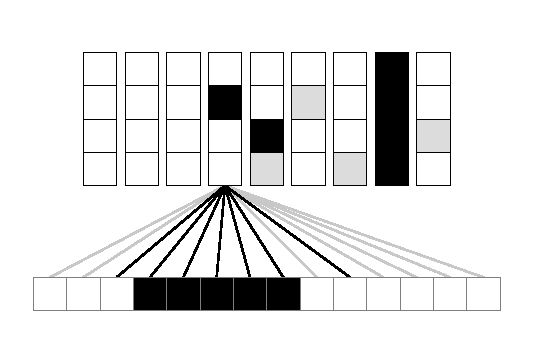
\includegraphics[width=0.53\textwidth]{algorithmDiagramStep3.eps}\hspace{1pc}%
	\begin{minipage}[b]{0.3\textwidth}
	\caption{Algorithm Step 3: This step calculates which cells to make predicting for the next time step. Note that none of the synapses for the cells have been shown.}\label{fig:algorithmDiagramStep3}
	\end{minipage}
\end{figure}

		\subsubsection{The classifier}
			The above three steps represent the core algorithm. However to form actual predictions of the next numerical input, a classifier is used. This classifier uses basic probabilistic methods to relate active cells to numerical input. As an aside, it is possible to generate a numerical prediction of the next input from the predicting cells. However Numenta has found that a classifier produces better results.
						 
	\subsection{Case study}
		%See notebook for detailed plan.
		This section provides a case study, showing the algorithm operating on some simple sine wave data. The data that will be used is shown in \ref{fig: exampleData}. Each step as detailed in the previous section will be shown for one sample in this data.
		
		The algorithm starts in a newly initialised state where it has learned no patterns. Samples from the data are fed in and the algorithm gradually learns to predict the next sample. The time step shown will be number NUMBER, after the algorithm has learned the data to the point where predictions are exact.
		
		
	
	\subsection{Noise characteristics}
%%%%%%%%%%%%%%%%%%%%%%%%%%%%%%%%%%%%%%%%%%%%%%%%%%
\section{Glitch Identification}
Intro/reasons for doing this (see big talk plan)
The hypothesis - how I imagined this method working (see big talk plan)
details - the experiment and the precise setup details
Results - The final Graph
Problems
 - overgeneralisation - and consequent investigation
 - low noise tolerance (signal indistinguishable when noise)
 - Trial of training with noise
Discussion - this is very simple but could be applied to other glitches / patterns
%%%%%%%%%%%%%%%%%%%%%%%%%%%%%%%%%%%%%%%%%%%%%%%%%%
\section{Additional Investigations}
\subsection{Gravitational Wave Detector Data}
\subsection{Beta Classification}
%%%%%%%%%%%%%%%%%%%%%%%%%%%%%%%%%%%%%%%%%%%%%%%%%%
\section{Conclusion}
Maybe some things like I had at the end of my talk - general issues in machine learning.
%%%%%%%%%%%%%%%%%%%%%%%%%%%%%%%%%%%%%%%%%%%%%%%%%%
\section*{References} 

This is some text. This is how you do citations: \cite{}. Type the first few letters and press F5.
%:FIG:matplotlibTest
\begin{center}
    \begin{figure}
            \includegraphics[width=\textwidth]{testMatplotlibPlot.pdf}
            \caption{A really exciting plot}
    \end{figure}
\end{center}

\end{document}


